\documentclass{standalone}
\usepackage{fancybox}
\usepackage{tikz}

\title{MergeSort-RecursionTree}
\author{Manuel Kirsch}
\date{}
\begin{document}

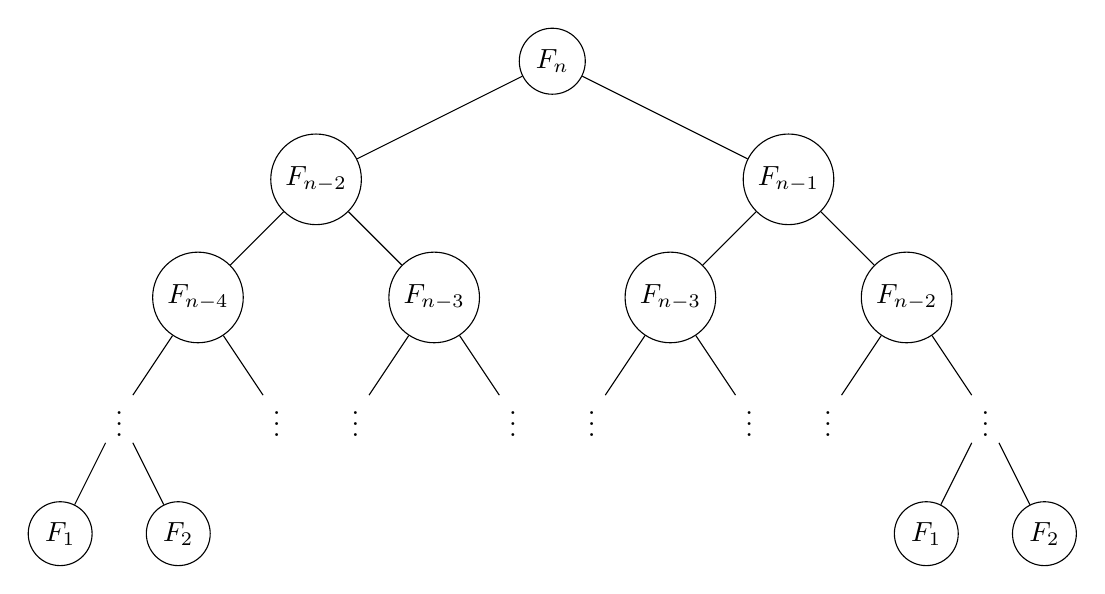
\begin{tikzpicture}[level/.style={sibling distance=60mm/#1}]
\node [circle,draw] (z){$F_n$}
  child {node [circle,draw] (a) {$F_{n-2}$}
    child {node [circle,draw] (b) {$F_{n-4}$}
      child {node {$\vdots$}
        child {node [circle,draw] (d) {$F_1$}}
        child {node [circle,draw] (e) {$F_2$}}
      } 
      child {node {$\vdots$}}
    }
    child {node [circle,draw] (g) {$F_{n-3}$}
      child {node {$\vdots$}}
      child {node {$\vdots$}}
    }
  }
  child {node [circle,draw] (j) {$F_{n-1}$}
    child {node [circle,draw] (k) {$F_{n-3}$}
      child {node {$\vdots$}}
      child {node {$\vdots$}}
    }
  child {node [circle,draw] (l) {$F_{n-2}$}
    child {node {$\vdots$}}
    child {node (c){$\vdots$}
      child {node [circle,draw] (o) {$F_1$}}
      child {node [circle,draw] (p) {$F_2$}
                }
              }
  }
};
\end{tikzpicture}

\end{document}
